¿Cuál es el valor de $x$ en la figura \ref{fig:findangle14}?

\begin{minipage}[t][][t]{0.35\textwidth}
    \begin{figure}[H]
        \centering
        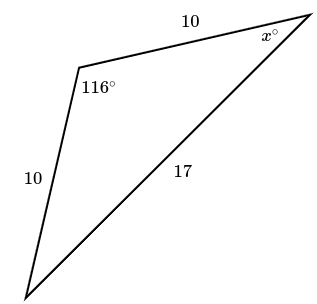
\includegraphics[width=0.65\linewidth]{../images/findangle14.png}
        \caption{}
        \label{fig:findangle14}
    \end{figure}
\end{minipage}\hfill
\begin{minipage}[t][][t]{0.65\textwidth}
    \begin{solutionbox}{5cm}\footnotesize
        \begin{wrapfigure}{r}{0.35\textwidth}
            \centering
            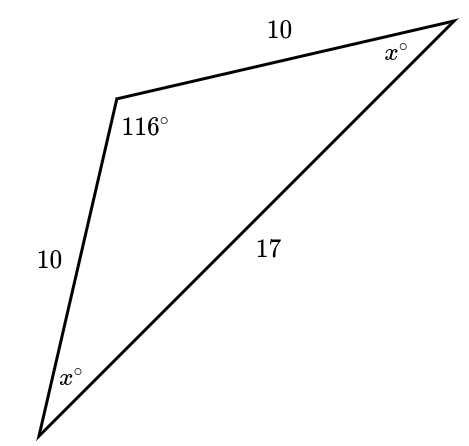
\includegraphics[width=0.85\linewidth]{../images/findangle14a.png}
            \caption{}
            \label{fig:findangle14a}
        \end{wrapfigure}
        Dado que tiene dos lados congruentes (aquellos cuya longitud es 10), el triángulo es isósceles. Los ángulos opuestos a los lados congruentes también son congruentes, por lo que el ángulo sin etiqueta mide $x^\circ$ (Ver Figura \ref{fig:findangle14a}).
        Los tres ángulos en un triángulo suman 180$^\circ$. Podemos escribir este enunciado como una ecuación:
        \[x^\circ + x^\circ + 116^\circ = 180^\circ \]
        \[\therefore x^\circ = \dfrac{180^\circ - 116^\circ}{2}  = 32^\circ\]
    \end{solutionbox}
\end{minipage}